\chapter{Vlakke figuren en lichamen}\label{ch:g2:shapes}

Vlakke figuren leven op papier; lichamen vullen je handen. In dit
hoofdstuk sorteren we vlakke figuren door zijden en hoeken te tellen,
testen we de rechte hoek met een gevouwen papieren hoekje, en ontmoeten
we de eerste lichamen --- met \omterm{def:g2:shapes:solids}{zijvlakken} die we allemaal al kennen.

\section{Vlakke figuren sorteren}

\begin{definition}[Recht van zijde of rond]\label{def:g2:shapes:sort}
Een figuur waarvan de rand alleen uit rechte zijden bestaat, is een
\emph{veelhoek}\index{veelhoek}: driehoek ($3$ zijden), vierhoek ($4$
zijden: vierkanten en rechthoeken zijn vierhoeken), vijfhoek ($5$),
zeshoek ($6$). Een figuur met een gebogen rand, zoals de cirkel, is
\emph{geen} veelhoek.
\end{definition}

\begin{omfigure}
\begin{tikzpicture}[scale=0.62]
  \draw[thick, fill=omDef!12] (0,0) -- (1.8,0) -- (0.9,1.5) -- cycle;
  \node[below, font=\small] at (0.9,-0.35) {$3$ zijden};
  \begin{scope}[xshift=3.2cm]
  \draw[thick, fill=omThm!12] (0,0) rectangle (1.7,1.5);
  \node[below, font=\small] at (0.85,-0.35) {$4$ zijden};
  \end{scope}
  \begin{scope}[xshift=6.6cm]
  % de vijfhoek is zo groot gekozen dat hij dezelfde hoogte (0..1.5) haalt
  \draw[thick, fill=omMeth!12] (0.95,0.67) +(90:0.83) -- +(162:0.83) --
    +(234:0.83) -- +(306:0.83) -- +(18:0.83) -- cycle;
  \node[below, font=\small] at (0.95,-0.35) {$5$ zijden};
  \end{scope}
  \begin{scope}[xshift=10.0cm]
  \draw[thick, fill=omProp!12] (0.75,0.75) circle (0.75);
  \node[below, font=\small] at (0.75,-0.35) {rond};
  \end{scope}
\end{tikzpicture}

{\small Sorteren op het aantal zijden. Het aantal hoeken is altijd
gelijk aan het aantal zijden.}
\end{omfigure}

\begin{method}[Een rechte hoek testen]\label{met:g2:shapes:rightangle}
Vouw een blad papier twee keer, zodat je een scherp hoekje krijgt ---
dat hoekje is een rechte hoek. Leg het in de hoek van een figuur:
\begin{enumerate}
  \item lopen de twee zijden van de figuur precies langs het gevouwen
        hoekje, dan is de hoek recht;
  \item is de hoek wijder of smaller, dan is hij niet recht.
\end{enumerate}
Een vierkant en een rechthoek hebben vier rechte hoeken.
\end{method}

\section{Natekenen op een raster}

\begin{method}[Een figuur natekenen]\label{met:g2:shapes:copy}
Teken op ruitjespapier een figuur hoekpunt voor hoekpunt na:
\begin{enumerate}
  \item kies een hoekpunt en zet het op het lege raster;
  \item tel de vakjes tot het volgende hoekpunt (``$3$ naar rechts, $2$
        naar boven'') en zet het;
  \item verbind de hoekpunten op volgorde en vergelijk met het
        voorbeeld.
\end{enumerate}
\end{method}

\begin{omfigure}
\begin{tikzpicture}[scale=0.5]
  \draw[gray!40] (0,0) grid (5,4);
  \draw[thick, omDef] (1,1) -- (4,1) -- (4,3) -- (2,3) -- cycle;
  \begin{scope}[xshift=7cm]
  \draw[gray!40] (0,0) grid (5,4);
  \draw[thick, omThm] (1,1) -- (4,1) -- (4,3) -- (2,3) -- cycle;
  \node[font=\footnotesize, omThm, below] at (2.5,-0.15) {de kopie};
  \end{scope}
\end{tikzpicture}

{\small Een figuur en zijn kopie, gemaakt door de vakjes tussen de
hoekpunten te tellen.}
\end{omfigure}

\section{Lichamen}

\begin{definition}[De eerste lichamen]\label{def:g2:shapes:solids}
Lichamen nemen ruimte in. Hun vlakke kanten zijn
\emph{zijvlakken}\index{zijvlak}:
\begin{itemize}
  \item de \emph{kubus}\index{kubus}: $6$ vierkante zijvlakken (een
        dobbelsteen);
  \item de \emph{balk}: $6$ rechthoekige zijvlakken (een pak
        ontbijtgranen);
  \item de \emph{cilinder}\index{cilinder}: twee ronde zijvlakken en een
        opgerolde zijkant (een blikje);
  \item de \emph{bol}: helemaal rond, geen enkel vlak zijvlak.
\end{itemize}
Lichamen en hun zijvlakken komen terug in \cref{ch:g5:solids}.
\end{definition}

\begin{omfigure}
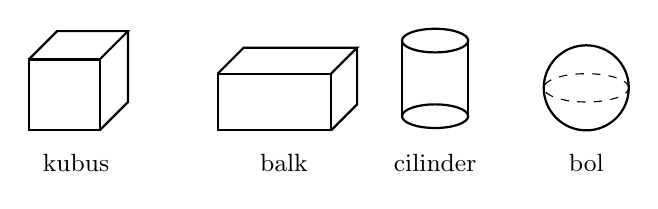
\begin{tikzpicture}[scale=0.6]
  \draw[thick] (0,0) rectangle (1.5,1.5);
  \draw[thick] (0,1.5) -- (0.6,2.1) -- (2.1,2.1) -- (1.5,1.5);
  \draw[thick] (2.1,2.1) -- (2.1,0.6) -- (1.5,0);
  \node[below, font=\small] at (1.0,-0.3) {kubus};
  \begin{scope}[xshift=4.0cm]
  \draw[thick] (0,0) rectangle (2.4,1.2);
  \draw[thick] (0,1.2) -- (0.55,1.75) -- (2.95,1.75) -- (2.4,1.2);
  \draw[thick] (2.95,1.75) -- (2.95,0.55) -- (2.4,0);
  \node[below, font=\small] at (1.4,-0.3) {balk};
  \end{scope}
  \begin{scope}[xshift=8.6cm]
  \draw[thick] (0,0.3) ellipse (0.7 and 0.25);
  \draw[thick] (-0.7,0.3) -- (-0.7,1.9);
  \draw[thick] (0.7,0.3) -- (0.7,1.9);
  \draw[thick] (0,1.9) ellipse (0.7 and 0.25);
  \node[below, font=\small] at (0,-0.3) {cilinder};
  \end{scope}
  \begin{scope}[xshift=11.8cm]
  \draw[thick] (0,0.9) circle (0.9);
  \draw[dashed] (0,0.9) ellipse (0.9 and 0.3);
  \node[below, font=\small] at (0,-0.3) {bol};
  \end{scope}
\end{tikzpicture}

{\small De eerste lichamen. Ga met je vinger over een \omterm{def:g2:shapes:solids}{kubus}: je voelt
$6$ vlakke \omterm{def:g2:shapes:solids}{zijvlakken} en scherpe ribben; een bol heeft er geen.}
\end{omfigure}

\section{Oefeningen}

\begin{exercise}[$\star$]\label{exo:g2:shapes:1}
Tel bij elke figuur de zijden en de hoeken en noem de figuur: een figuur
met $5$ zijden; een figuur met $3$ hoeken; een ronde figuur.
\end{exercise}

\begin{exercise}[$\star$]\label{exo:g2:shapes:2}
Sorteer in ``\omterm{def:g2:shapes:sort}{veelhoek}'' of ``geen \omterm{def:g2:shapes:sort}{veelhoek}'': een vierkant; een cirkel;
een driehoek; een zeshoek.
\end{exercise}

\begin{exercise}[$\star$]\label{exo:g2:shapes:3}
Maak een hoekentester door papier te vouwen. Zoek drie rechte hoeken in
de kamer, en één hoek die niet recht is.
\end{exercise}

\begin{exercise}[$\star$]\label{exo:g2:shapes:4}
Hoeveel rechte hoeken heeft een vierkant? En een rechthoek? Hoeveel kan
een driehoek er hoogstens hebben? (Probeer er een met twee te tekenen.)
\end{exercise}

\begin{exercise}[$\star$]\label{exo:g2:shapes:5}
Teken op ruitjespapier een rechthoek van $4$ vakjes breed en $2$ hoog
na, en daarna een driehoek met een basis van $3$ vakjes.
\end{exercise}

\begin{exercise}[$\star$]\label{exo:g2:shapes:6}
Noem het lichaam: een dobbelsteen; een blikje soep; een voetbal; een
schoenendoos.
\end{exercise}

\begin{exercise}[$\star$]\label{exo:g2:shapes:7}
Hoeveel \omterm{def:g2:shapes:solids}{zijvlakken} heeft een \omterm{def:g2:shapes:solids}{kubus}? Welke vorm heeft elk \omterm{def:g2:shapes:solids}{zijvlak}?
Hoeveel \omterm{def:g2:shapes:solids}{zijvlakken} heeft een balk?
\end{exercise}

\begin{exercise}[$\star$]\label{exo:g2:shapes:8}
Welke lichamen kunnen rollen: de \omterm{def:g2:shapes:solids}{kubus}, de balk, de bol, de \omterm{def:g2:shapes:solids}{cilinder}?
Waarom?
\end{exercise}

\begin{exercise}[$\star$]\label{exo:g2:shapes:9}
Een figuur heeft $6$ zijden. Hoe heet die? Hoeveel hoeken heeft hij?
\end{exercise}

\begin{exercise}[$\star\star$]\label{exo:g2:shapes:10}
Teken op ruitjespapier een huis: een vierkant voor de muur
($4 \times 4$) met een driehoek als dak erbovenop. Hoeveel zijden en
hoeken heeft de buitenrand van het hele huis?
\end{exercise}
